\documentclass{article}

\usepackage[preprint]{neurips_2025}
\usepackage[utf8]{inputenc}
\usepackage[T1]{fontenc}
\usepackage{hyperref}
\usepackage{url}
\usepackage{booktabs}
\usepackage{amsfonts}
\usepackage{amsmath, amssymb, amsthm}
\usepackage{mathtools}
\usepackage{algorithm}
\usepackage{algorithmic}
\usepackage{graphicx}
\usepackage{xcolor}
\usepackage{tikz}
\usetikzlibrary{arrows.meta, positioning, fit, backgrounds, shapes}
\usepackage{subcaption}
\usepackage{multirow}
\usepackage{enumitem}

% ---- theorem environments ----
\newtheorem{definition}{Definition}
\newtheorem{proposition}{Proposition}
\newtheorem{remark}{Remark}
\newtheorem{assumption}{Assumption}

% ---- macros ----
\newcommand{\cG}{\mathcal{G}}
\newcommand{\R}{\mathbb{R}}
\newcommand{\E}{\mathbb{E}}
\renewcommand{\do}{\mathrm{do}}
\newcommand{\Pa}{\mathrm{Pa}}
\newcommand{\An}{\mathrm{An}}
\newcommand{\De}{\mathrm{De}}
\newcommand{\GP}{\mathcal{GP}}
\newcommand{\QCBO}{\textsc{QCBO}}
\newcommand{\CBO}{\textsc{CBO}}
\newcommand{\BO}{\textsc{BO}}
\newcommand{\Gq}{\mathcal{G}^{\pi}}
\newcommand{\Gg}{\mathcal{G}}
\newcommand{\Ga}{\mathcal{G}^\alpha}
\newcommand{\ESpi}{\mathfrak{S}^{\pi}}

% ==========================================
\title{Quotient Causal Bayesian Optimization}

\author{Anonymous}

\begin{document}
\maketitle

% ==========================================
\begin{abstract}
Causal Bayesian optimization (CBO) finds the intervention that optimizes a
target variable, but existing methods assume the full causal DAG over all
manipulable variables is known --- a level of structural knowledge
practitioners rarely have. We introduce Quotient CBO (\QCBO{}), which
coarsens the manipulable variables and requires only a \emph{partition} of
them into clusters together with the cluster-level graph (a C-DAG):
identification, exploration-set construction, and the causal GP prior are all
derived from the quotient structure. We frame this as a modeling contribution
and prove the structural robustness it confers --- \emph{any} misspecification
of edges inside a cluster is provably invisible to \QCBO{} --- together with a
price-of-coarsening characterization: the attainable optimum degrades
monotonically along the coarsening lattice, with equality exactly when an
optimal intervention set is a union of clusters. On the standardized
\textsc{CausalBO} benchmark (a curated set of hard-intervention SCMs, scored
with the community GAP / PA-GAP metrics) and a purpose-built
confounded-cluster benchmark, \QCBO{} at the identity partition coincides with
full-knowledge CBO by construction, coarse partitions trade optimality for
robustness exactly as predicted, and an intra-cluster misspecification that
structurally damages fine-grained CBO (deleting its optimal intervention
target from the exploration set) leaves \QCBO{}'s trajectories byte-for-byte
unchanged.
\end{abstract}

% ==========================================
\section{Introduction}
\label{sec:intro}

Causal Bayesian optimization \citep{aglietti2020causal} unifies two ideas:
when the variable $Y$ we wish to optimize sits inside a causal system, the
right search space is the space of \emph{interventions}
$\do(X_S=\mathbf{x}_S)$, and observational data plus the causal graph yield
informative priors over the interventional response surfaces. The catch is
the input requirement. CBO and its descendants
\citep{aglietti2021dynamic,aglietti2023constrained,sussex2023model} assume
the full DAG over all observables --- every edge, every latent confounder
--- is specified correctly. Practitioners typically have something weaker
and more reliable: they know the \emph{groups}. A clinician treats the
medications a patient takes (e.g.\ statin and aspirin) as one ``treatment''
lever without committing to their pharmacological interactions; a reef
ecologist distinguishes nutrient/chemistry stressors from temperature/depth
forcing without specifying the edges \emph{within} either subsystem.
The graph-free end of the spectrum is served by methods that learn
structure online \citep{mukherjee2024gacbo,branchini2023causal} at a heavy
per-trial cost. The middle of the spectrum --- cluster-level knowledge ---
has well-developed identification theory
\citep{anand2023cdag,ferreira2025cdmg,wahl2024foundations} but, to our
knowledge, no optimization method.

\QCBO{} fills this gap. The practitioner supplies a partition $\pi$ of the
manipulable variables; \QCBO{} builds the quotient graph $\Gq$ (a C-DAG over
clusters, with bidirected edges absorbing latent confounding via the latent
projection of \citealp{lee2019latent}), restricts exploration to
cluster-level interventions whose effects are identifiable from $\Gq$, and
uses the identified cluster-level do-calculus estimates as GP prior means.
The central structural insight is that this construction never looks inside
a cluster:

\paragraph{Contributions.}
\begin{itemize}[leftmargin=1.2em,itemsep=1pt,topsep=2pt]
  \item We formalize \QCBO{}: Bayesian optimization over cluster-level
  interventions with identification performed on the C-DAG by a complete
  algorithm \citep{shpitser2006identification}, an
  identifiability-gated exploration set, and a two-tier causal GP prior
  (\S\ref{sec:ccbo}).
  \item As a \emph{modeling} contribution (not a claim of new estimation
  theory), we show what the construction buys: an \emph{intra-cluster
  invariance} property (Prop.~\ref{prop:invariance}) --- every quantity
  \QCBO{} computes is invariant to arbitrary edge misspecification within
  clusters --- and a \emph{price-of-coarsening} characterization
  (Prop.~\ref{prop:price}): the attainable optimum is monotone along the
  coarsening lattice, with an exact condition for losslessness. We also prove
  that validity is \emph{not} monotone under refinement
  (Prop.~\ref{prop:refinement_validity}: refining a valid partition can
  introduce a cyclic quotient), while exploration and identifiability are
  monotone under valid refinements (Prop.~\ref{prop:refinement}). The
  propositions have short, self-contained proofs (\S\ref{sec:theory}); per-dataset
  partitions and C-DAGs are in Appendix~\ref{app:datasets}.
  \item We evaluate on the standardized \textsc{CausalBO} benchmark
  \citep{anonymous2026cbobench} --- a curated subset of hard-intervention SCMs
  (ToyGraph, Synthetic, Synthetic-2, Healthcare, Epidemiology, Ecology),
  scored with its GAP / PA-GAP metrics and oracle optima --- and on a
  purpose-built confounded-cluster benchmark that separates two damage regimes
  of DAG misspecification: prior bias (recoverable by the BO loop) and
  exploration-set damage (unrecoverable). We verify that coarsening is
  provably immune to both when the misspecification is intra-cluster
  (\S\ref{sec:experiments}).
\end{itemize}


% ==========================================
\section{Background}
\label{sec:background}

\paragraph{SCMs and interventions.}
A structural causal model $\mathcal{M}=\langle
\mathbf{U},\mathbf{V},\mathcal{F},P(\mathbf{U})\rangle$ induces a
distribution over observables $\mathbf{V}$ and, for any $S \subseteq
\mathbf{V}$, interventional distributions $P(\cdot \mid \do(X_S =
\mathbf{x}_S))$ obtained by replacing the mechanisms of $X_S$ with
constants \citep{pearl2009causality}. The induced graph $\Gg$ has a
directed edge per functional argument and a bidirected edge per shared
latent; projecting out latents yields an ADMG over $\mathbf{V}$
\citep{lee2019latent}.

\paragraph{Causal Bayesian optimization.}
Given manipulable variables $\mathbf{X} \subseteq \mathbf{V}$ and target
$Y$, CBO \citep{aglietti2020causal} solves
\begin{equation}
  \label{eq:cbo_obj}
  (S^*, \mathbf{x}^*) = \arg\min_{\substack{S \in \mathfrak{S} \\ \mathbf{x}_S \in \mathcal{X}_S}}
  \E\!\left[Y \mid \do(X_S = \mathbf{x}_S)\right],
\end{equation}
maintaining one GP per \emph{candidate intervention set} $S$ in an exploration
set $\mathfrak{S}$, with prior mean given by the do-calculus estimate of
$\E[Y \mid \do(X_S=\mathbf{x}_S)]$ from observational data and the assumed
graph, and selecting $(S,\mathbf{x})$ by expected improvement
\citep{garnett2023bayesian}. We use ``candidate intervention set'' (or, loosely
and only by analogy to the causal-bandit lineage that supplies the pruning
below, ``arm'') for a member of $\mathfrak{S}$; each is itself a
\emph{continuous} BO sub-problem over $\mathbf{x}_S$, not a single bandit arm.
The exploration set is pruned structurally (MIS/POMIS;
\citealp{lee2018structural}); both the pruning and the priors are functions of
the assumed graph, which is where misspecification enters.

\paragraph{Coarsening and C-DAGs.}
\begin{definition}[Coarsening~\citep{madaleno2026coarsening}]
\label{def:coarsening}
Given a DAG $\Gg$ on $\mathbf{V}$, a \textbf{coarsening} is a partition
$\pi=\{C_1,\ldots,C_{d'}\}$ of $\mathbf{V}$ such that the induced quotient
$\Gq$ --- nodes $\{C_1,\ldots,C_{d'}\}$, edge $C_k\to C_\ell$ ($k \neq
\ell$) iff $\exists\, V_i\in C_k, V_j\in C_\ell$ with $V_i\to V_j$ in
$\Gg$ --- is acyclic. $\pi$ is then called \emph{valid}.
\end{definition}
For ADMGs the quotient additionally carries $C_k \leftrightarrow C_\ell$
iff some $V_i \in C_k$, $V_j \in C_\ell$ are connected by a bidirected
edge; intra-cluster bidirected edges are dropped. The resulting object is a
C-DAG in the sense of \citet{anand2023cdag}, who prove that do-calculus on
the C-DAG is sound and complete for the equivalence class of fine-grained
graphs that quotient to it. Markov properties transfer to the cluster
level, but faithfulness does not \citep{wahl2024foundations}.


% ==========================================
\section{Quotient Causal Bayesian Optimization}
\label{sec:ccbo}

\subsection{Setup}
\label{sec:setup}

The practitioner partitions only the manipulable variables: $\pi$ is a
partition of $\mathbf{X}$, the target $Y$ is kept as a singleton, and every
non-manipulable observable remains an atomic (singleton) vertex of the
quotient. Mixing manipulable and non-manipulable variables in one cluster
is disallowed --- intervening on a cluster must be a physically executable
action. Hidden confounders are first projected out of $\Gg$
\citep{lee2019latent}, giving an ADMG $\Gg^{*}$ over observables; the
coarsened graph $\Gq$ is the quotient of $\Gg^{*}$ under $\pi$ (plus
atomic vertices), and validity (acyclicity of the directed part) is
checked. Intervening on a cluster $C_k$ means jointly setting all of its
members: $\do(C_k = \mathbf{c}_k)$. The candidate exploration set contains
all unions of at most $m$ clusters:
\begin{equation}
  \label{eq:ccbo_exploration}
  \ESpi_{0} = \Bigl\{\, \bigcup_{C_k \in \mathcal{S}} C_k
  \;\Big|\; \emptyset \neq \mathcal{S} \subseteq \pi,\;
  |\mathcal{S}| \leq m \,\Bigr\}.
\end{equation}

\begin{remark}[Intervention granularity]
\label{rem:granularity}
Merging manipulable variables coarsens the \emph{action space}: \QCBO{}
can only set a cluster jointly, never a strict subset of it. This is the
mechanism behind both the robustness (\S\ref{sec:theory}) and the price
(Prop.~\ref{prop:price}) of coarsening.
\end{remark}

\subsection{Identifiability-gated exploration and the two-tier prior}
\label{sec:causal_prior}

For each candidate $S \in \ESpi_0$ we pose the cluster-level query $P(Y
\mid \do(S))$ on $\Gq$ and run the complete ID algorithm of
\citet{shpitser2006identification} (via \texttt{ananke};
\citealp{lee2023ananke}). Following the arm-pruning tradition of
structural causal bandits \citep{lee2018structural}, \QCBO{} \emph{commits
to its structural beliefs}: the exploration set $\ESpi$ keeps exactly the
candidates whose effect is identifiable from $\Gq$,
\begin{equation}
  \label{eq:es_gate}
  \ESpi = \{\, S \in \ESpi_0 \;:\; P(Y \mid \do(S)) \text{ identifiable
  from } \Gq \,\}.
\end{equation}
This gate is exact (ID is complete on the C-DAG, and identification from
$\Gq$ is sound for every fine graph in its class;
\citealp{anand2023cdag}), and it is what transmits structural
misspecification into behaviour: a wrong assumed graph keeps or removes
\emph{arms}, not just priors (\S\ref{sec:robustness}). The alternative
design --- exploring non-identified arms under an uninformative prior ---
trades this structural damage for exploration overhead; we discuss it in
\S\ref{sec:limitations}.

For $S \in \ESpi$, the GP prior mean is constructed in two tiers. The ID
gate guarantees a non-parametric formula exists; our \emph{estimator}
instantiates it as a cascade of GP-based plug-ins (backdoor adjustment
$\to$ front-door $\to$ $g$-computation) on the bidirected-edge expansion
of $\Gq$. The cascade is sound but not complete, so on the rare queries it
cannot instantiate we fall back to the observational mean:
\begin{equation}
  \label{eq:two_tier_prior}
  \mu_0^S(\mathbf{x}_S) = \begin{cases}
    \hat{\E}[Y \mid \do(X_S = \mathbf{x}_S)] & \text{estimator cascade
    instantiates the ID formula,} \\
    \bar{Y}_{\mathrm{obs}} & \text{otherwise (logged as a diagnostic).}
  \end{cases}
\end{equation}
Because clusters are manipulable-only and interventions assign full
clusters, the cluster-level formulas expand exactly into fine-grained
regressions on observational data --- no sub-cluster heuristic is
involved.

\begin{assumption}[Valid partition]
\label{ass:valid}
The practitioner supplies a partition $\pi$ of $\mathbf{X}$ whose quotient
$\Gq$ is acyclic. (Validity is checkable from cluster-level knowledge
alone and is verified by the implementation.)
\end{assumption}

\begin{assumption}[Estimator-completeness boundary]
\label{ass:id_scheme}
The ID gate (Eq.~\ref{eq:es_gate}) is complete; the GP estimator cascade
behind Eq.~\eqref{eq:two_tier_prior} is sound but not complete. Queries
that pass the gate but miss the cascade are reported and receive the
uninformative tier. In all benchmarks of \S\ref{sec:experiments} this set
is empty.
\end{assumption}

\subsection{Algorithm}

\begin{algorithm}[t]
\caption{\QCBO: Quotient Causal Bayesian Optimization}
\label{alg:ccbo}
\begin{algorithmic}[1]
\REQUIRE Assumed graph $\Gg$ (or directly $\Gq$); partition $\pi$ of
$\mathbf{X}$; target $Y$; budget $T$; observational data
$\mathcal{D}_{\mathrm{obs}}$; cluster budget $m$.
\STATE $\Gg^* \leftarrow$ latent projection of $\Gg$;\quad $\Gq
\leftarrow$ quotient of $\Gg^*$ under $\pi$; check acyclicity.
\STATE Build $\ESpi$ via Eqs.~\eqref{eq:ccbo_exploration},
\eqref{eq:es_gate} (one complete-ID call per candidate).
\STATE For each $S \in \ESpi$: fit the prior $\mu_0^S$ via
Eq.~\eqref{eq:two_tier_prior} on $\mathcal{D}_{\mathrm{obs}}$.
\STATE Collect initial interventional data $\mathcal{D}_0$.
\FOR{$t = 1, \ldots, T$}
  \STATE Update GP posteriors $(\mu_t^S, k_t^S)$ for all $S \in \ESpi$.
  \STATE $(S_t, \mathbf{x}_t) \leftarrow \arg\max_{S,\mathbf{x}}
  \mathrm{EI}_{S,t}(\mathbf{x}) / \mathrm{cost}(S,\mathbf{x})$.
  \STATE Intervene, observe $y_t$; update $\mathcal{D}_t$.
\ENDFOR
\RETURN $(S_{t^*}, \mathbf{x}_{t^*})$ where $t^* = \arg\min_t y_t$.
\end{algorithmic}
\end{algorithm}


% ==========================================
\section{Theoretical properties}
\label{sec:theory}

These results are a \emph{modeling} contribution rather than new estimation
theory: \QCBO{}'s inputs are the quotient $\Gq$ and data, and the quotient is
by construction blind to intra-cluster edges. The propositions below make
precise what that design buys (invariance, Prop.~\ref{prop:invariance}), what
it costs (price of coarsening, Prop.~\ref{prop:price}), and where it is subtle
(validity is not refinement-monotone, Prop.~\ref{prop:refinement_validity}).
The proofs are short, compositional arguments about quotients and set
inclusion --- which is exactly why the invariance is \emph{structural}: no
intra-cluster hypothesis is even representable.

Throughout, $\pi, \pi'$ are manipulable-only partitions as in
\S\ref{sec:setup}; $\pi_\top$ denotes the identity (all-singleton)
partition; $\pi'$ \emph{refines} $\pi$ ($\pi' \preceq \pi$) iff every
cluster of $\pi'$ is contained in a cluster of $\pi$.

\begin{proposition}[Identity recovery]
\label{prop:identity}
Under $\pi=\pi_\top$, $\Gq = \Gg^{*}$ and $\ESpi_0$ is the set of all
subsets of $\mathbf{X}$ of size at most $m$; \QCBO{} reduces to \CBO{}
with an identifiability-gated exploration set.
\end{proposition}
\begin{proof}[Proof sketch]
Singleton clusters make the quotient map the identity, and unions of at most
$m$ singletons are exactly the size-$\le m$ subsets (full proof
App.~\ref{app:proofs}).
\end{proof}

\begin{proposition}[Invariance to intra-cluster misspecification]
\label{prop:invariance}
Let $\pi$ be valid for $\Gg$ and let $\Gg'$ differ from $\Gg$ by an
arbitrary set of insertions, deletions, or reversals of edges (directed or
bidirected) whose endpoints lie within a single cluster of $\pi$, with
$\Gg'$ acyclic. Then $(\Gg')^{\pi} = \Gq$, and consequently the
exploration set (Eq.~\ref{eq:es_gate}), every identification formula, every
prior (Eq.~\ref{eq:two_tier_prior}), and --- given the same data and seeds
--- the entire \QCBO{} trajectory are identical under $\Gg$ and $\Gg'$.
\end{proposition}
\begin{proof}[Proof sketch]
Latent projection touches only latent vertices, and the quotient keeps a
cluster-level edge iff some fine edge crosses \emph{distinct} clusters; so
intra-cluster changes leave $\Gq$ --- and every object derived from it
($\ESpi$, ID formulas, priors) --- fixed (full proof App.~\ref{app:proofs}).
\end{proof}

\begin{remark}[What invariance buys]
\label{rem:structural_robustness}
Prop.~\ref{prop:invariance} is a statement about the \emph{method}, not
about estimation error: \QCBO{} cannot even represent an intra-cluster
hypothesis, so no intra-cluster mistake can affect it. \S\ref{sec:robustness}
shows the same mistakes can structurally damage fine-grained CBO by
deleting its best arm.
\end{remark}

\begin{proposition}[Validity is not refinement-monotone]
\label{prop:refinement_validity}
There exist a valid partition $\pi$ and a refinement $\pi'\preceq\pi$ whose
quotient $\mathcal{G}^{\pi'}$ is cyclic; hence refinement does not preserve
validity. Validity is nonetheless decidable from cluster-level structure
alone --- $\pi'$ is valid iff the directed part of $\mathcal{G}^{\pi'}$ is
acyclic (Def.~\ref{def:coarsening}) --- so it must be re-verified after each
refinement.
\end{proposition}
\begin{proof}[Proof sketch]
The fine edges $a_1\to b_1$ and $b_2\to a_2$ are intra-cluster under the
coarsest partition but expose a $2$-cycle $A\rightleftarrows B$ once
$\{a_1,a_2\},\{b_1,b_2\}$ are split; decidability is the acyclicity clause of
Def.~\ref{def:coarsening} (full proof App.~\ref{app:proofs}).
\end{proof}

\begin{proposition}[Monotonicity under valid refinement]
\label{prop:refinement}
Let $\pi' \preceq \pi$ with both valid, and take $m = \infty$ in
Eq.~\eqref{eq:ccbo_exploration}. Then (i) $\ESpi_0 \subseteq
\mathfrak{S}^{\pi'}_{0}$; (ii) every $S \in \ESpi$ is also in
$\mathfrak{S}^{\pi'}$, i.e.\ effects identifiable from $\Gq$ remain
identifiable from $\mathcal{G}^{\pi'}$, with the same functional.
\end{proposition}
\begin{proof}[Proof sketch]
Unions of $\pi$-clusters are unions of $\pi'$-clusters, and quotienting is
compositional, so a functional identifying $\E[Y\mid\do(S)]$ across the class
compatible with $\Gq$ works a fortiori on the smaller class compatible with
$\mathcal{G}^{\pi'}$ \citep{anand2023cdag} (full proof App.~\ref{app:proofs}).
\end{proof}

\begin{proposition}[Price of coarsening]
\label{prop:price}
Let $\mu^*(S) = \min_{\mathbf{x}_S} \E[Y \mid \do(X_S=\mathbf{x}_S)]$ and
$V(\pi) = \min_{S \in \ESpi_0} \mu^*(S)$, with $m=\infty$. For any valid
$\pi' \preceq \pi$:
\[
V(\pi_\top) \;\le\; V(\pi') \;\le\; V(\pi),
\]
and $V(\pi) = V(\pi_\top)$ iff some optimizer $S^*$ of
Eq.~\eqref{eq:cbo_obj} is a union of $\pi$-clusters.
\end{proposition}
\begin{proof}[Proof sketch]
The exploration sets nest, $\ESpi_0\subseteq\mathfrak{S}^{\pi'}_0\subseteq
2^{\mathbf{X}}\setminus\{\emptyset\}$, so the minima are monotone; equality
holds iff the unrestricted argmin already lies in $\ESpi_0$ (full proof
App.~\ref{app:proofs}).
\end{proof}

\begin{remark}[Damage taxonomy for misspecification]
\label{rem:taxonomy}
Under the gated design (Eq.~\ref{eq:es_gate}), a wrong assumed graph can
hurt in two distinct ways. \emph{Tier-1 (prior bias):} the arm survives
but its prior mean is wrong; expected improvement wastes evaluations, and
the interventional data eventually correct it --- the damage is a
convergence-speed cost. \emph{Tier-2 (arm damage):} the wrong graph flips
the identifiability verdict, deleting an arm from $\ESpi$ (or admitting a
spurious one); if the deleted arm contained the optimum, no amount of data
recovers it. Prop.~\ref{prop:invariance} says coarsening is immune to both
tiers whenever the misspecified edges are intra-cluster.
\end{remark}


% ==========================================
\section{Related work}
\label{sec:related}

\begin{table}[t]
  \centering
  \caption{Positioning of \QCBO{} against the nearest methods.}
  \label{tab:related}
  \vspace{4pt}
  \small
  \begin{tabular}{@{}llll@{}}
    \toprule
    \textbf{Method} & \textbf{What is learned} & \textbf{Structural prior assumed} & \textbf{Search space} \\
    \midrule
    CBO~\citep{aglietti2020causal}    & nothing (oracle DAG) & full DAG & MIS \\
    GACBO~\citep{mukherjee2024gacbo}  & posterior over DAGs & DAG family & union of MIS \\
    Durand et al.~\citep{durand2025unknown} & $\Pa(Y) \subseteq \mathbf{X}$ & $Y$ leaf & $\mathbf{X}$ \\
    Park et al.~\citep{park2025dmis} & PAG $\to$ MAG & MEC & partial $\mathbf{X}$ \\
    SCB~\citep{lee2018structural}     & nothing (oracle DAG) & full DAG & POMIS (atomic) \\
    \midrule
    \QCBO{} (ours) & nothing & partition of $\mathbf{X}$ + C-DAG & ID-gated cluster unions \\
    \bottomrule
  \end{tabular}
\end{table}

The recent survey of \citet{anonymous2026cbobench} organizes the CBO
landscape along four design axes --- graph knowledge, intervention
representation, surrogate, and decision rule --- and its ``unknown causal
structure'' family contains only methods that \emph{learn} or \emph{average}
graphs (CEO, GACBO, Durand et al.). \QCBO{} occupies an unfilled cell on the
graph-knowledge axis: it neither assumes the full DAG nor learns one, but
takes a coarser, more reliable input (a partition + C-DAG) and identifies on
the quotient. It also speaks directly to two open problems the survey
highlights --- robustness to hidden confounding and scalable unknown-graph
optimization. Concretely, methods that relax CBO's full-graph requirement
either learn structure online --- GACBO maintains a posterior over plausible
DAGs at substantial per-trial cost \citep{mukherjee2024gacbo}, local-discovery
CBO learns around $Y$ \citep{branchini2023causal}, and
\citet{durand2025unknown} identify $\Pa(Y)$ under a $Y$-leaf assumption and
search over $\mathbf{X}$ --- or assume an equivalence class is known
\citep{park2025dmis}. Even the most recent CBO work that broadens the action
space, contextual CBO \citep{arsenyan2026contextual}, still assumes the full
graph is given. \QCBO{} instead assumes \emph{less structure of a different
kind}: a partition with cluster-level edges, learning no edges at all. The
identification side of this regime is established --- C-DAG do-calculus
\citep{anand2023cdag}, its extension to C-DMGs over ADMGs
\citep{ferreira2025cdmg}, cluster-level Markov properties
\citep{wahl2024foundations}, and recent work on relaxing partition
admissibility \citep{tikka2025relaxing} and on C-DAGs as background knowledge
for discovery \citep{ll2025cdagdiscovery} --- but none of these perform
optimization.

\paragraph{Multi-fidelity and abstraction-based BO.}
Closest in spirit is the concurrent position paper of
\citet{zeitler2025mfacbo}, which proposes MFACBO --- a hybrid of CBO and
multi-information-source BO~\citep{poloczek2017multi} unified through
approximate causal abstraction~\citep{beckers2019approximate}. MFACBO
coarsens the \emph{outcome} ($Y_{\text{low}}$ as a cheap, biased proxy of
$Y_{\text{high}}$); \QCBO{} is complementary in that it coarsens the
\emph{manipulable inputs} into cluster-level interventions and exploits
identification on the resulting C-DAG. The two axes are orthogonal and
could be combined in a single surrogate; we leave the hybrid to future
work.


% ==========================================
\section{Experiments}
\label{sec:experiments}

\subsection{Setup}
\label{sec:exp_setup}

\textbf{Standardized benchmark.} Our main evaluation uses the curated
hard-intervention subset of the \textsc{CausalBO} benchmark
\citep{anonymous2026cbobench}: \emph{ToyGraph} and \emph{Synthetic-2}
(chains $X\!\to\!Z\!\to\!Y$), \emph{Synthetic} (the six-observable graph of
\citealp{aglietti2020causal} with latents $U_1\!\to\!\{A,Y\}$,
$U_2\!\to\!\{B,Y\}$; manipulable $\{B,D,E\}$), \emph{Healthcare} (statin/aspirin
$\to$ PSA, with observed age/BMI confounding), \emph{Epidemiology} (an HIV SCM,
manipulable $\{L,B\}$), and \emph{Ecology} (a fitted coral-reef SCM, manipulable
$\{N,O,C,T,D\}$). We run each through the benchmark's own CBO loop and score the
exported best-so-far trajectories with its \emph{GAP} and \emph{PA-GAP}
metrics against its shipped oracle optima $y^*$ --- so our numbers are directly
comparable to the benchmark's other methods. For each dataset we use the
identity partition (\QCBO{}-finest, which by Prop.~\ref{prop:identity}
\emph{is} \CBO{}) and one domain-meaningful coarse partition; the partitions
and C-DAGs are listed in Appendix~\ref{app:datasets}.

\textbf{Controlled robustness benchmarks.} The standardized datasets assume
causal sufficiency or place confounders away from manipulable pairs, so none
exhibits the structure that drives misspecification damage. We therefore use
two controlled SCMs for the robustness study: \emph{CompleteGraph} (=Synthetic,
for Tier-1 prior bias) and a purpose-built \emph{ConfoundedCluster} ``bow''
benchmark (for Tier-2 arm deletion): manipulable $\{A,B,C\}$, latent
$U\!\to\!\{B,C\}$ giving $\mathrm{corr}(B,C)\!\approx\!0.70$, with the strongest
lever $\do(B)$.

\textbf{Protocol.} On the standardized benchmark we follow its protocol
($T{=}100$ trials, unit costs, the single-draw SEM objective and offline $y^*$),
report GAP / PA-GAP at $100/50/20$ trials over $5$ seeds, and route every
method's trajectory through the same scorer. The exploration-set cap matches
the benchmark's own ($m=\min(5,|\mathbf{X}|)$: all interventions on up to $m$
manipulable variables), so at $\pi_\top$ \QCBO{}-finest searches exactly
\CBO{}'s candidate set. On the controlled benchmarks all
methods share the same seeds, initial-data budget, trial budget, and
per-benchmark cluster cap $m$; a fairness check enforces identical trajectory
lengths, seed coverage, and initial-budget across methods. Reported
uncertainties are standard errors (sample s.d., $\mathrm{ddof}{=}1$).

\begin{table}[t]
  \centering
  \caption{\QCBO{} on the curated \textsc{CausalBO} benchmark: final $Y$,
  GAP, and PA-GAP (mean $\pm$ s.e., 5 seeds, 100 trials), scored by the
  benchmark's own pipeline against its oracle $y^*$. \QCBO{}-finest is
  \CBO{} on the full DAG (Prop.~\ref{prop:identity}); \QCBO{}-coarse uses the
  domain partition of Appendix~\ref{app:datasets}. GAP is improvement relative
  to each method's initial incumbent and $y^*$ is an extreme oracle reference,
  so the values read as a relative ranking rather than an attainment fraction
  (see Limitations). Auto-generated; the
  included file ends with its own \texttt{\textbackslash bottomrule}.}
  \label{tab:benchmark}
  \vspace{4pt}
  \small
  \begin{tabular}{@{}llccc@{}}
    \toprule
    \textbf{Dataset} & \textbf{Method} & \textbf{Final $Y$} &
    \textbf{GAP} & \textbf{PA-GAP} \\
    \midrule
    \multirow{2}{*}{ToyGraph} & CBO ($=$\QCBO{}-finest) & $-2.172 \pm 0.000$ & $0.390 \pm 0.056$ & $0.176 \pm 0.065$ \\
 & \QCBO{}-coarse & $-2.172 \pm 0.000$ & $0.453 \pm 0.068$ & $0.238 \pm 0.058$ \\
\midrule
\multirow{2}{*}{Synthetic-2} & CBO ($=$\QCBO{}-finest) & $-1.856 \pm 0.000$ & $0.370 \pm 0.036$ & $0.082 \pm 0.029$ \\
 & \QCBO{}-coarse & $-0.511 \pm 0.000$ & $0.490 \pm 0.007$ & $0.018 \pm 0.006$ \\
\midrule
\multirow{2}{*}{Synthetic} & CBO ($=$\QCBO{}-finest) & $-1.739 \pm 0.212$ & $0.127 \pm 0.109$ & $0.018 \pm 0.017$ \\
 & \QCBO{}-coarse & $-1.737 \pm 0.257$ & $0.317 \pm 0.099$ & $0.051 \pm 0.015$ \\
\midrule
\multirow{2}{*}{Healthcare} & CBO ($=$\QCBO{}-finest) & $5.352 \pm 0.041$ & $0.208 \pm 0.128$ & $0.011 \pm 0.009$ \\
 & \QCBO{}-coarse & $5.329 \pm 0.015$ & $0.360 \pm 0.071$ & $0.033 \pm 0.010$ \\
\midrule
\multirow{2}{*}{Epidemiology} & CBO ($=$\QCBO{}-finest) & $-2.344 \pm 0.031$ & $0.542 \pm 0.106$ & $0.168 \pm 0.044$ \\
 & \QCBO{}-coarse & $-2.300 \pm 0.026$ & $0.473 \pm 0.058$ & $0.254 \pm 0.027$ \\
\midrule
\multirow{2}{*}{Ecology} & CBO ($=$\QCBO{}-finest) & $5.023 \pm 0.036$ & $0.099 \pm 0.067$ & $0.001 \pm 0.001$ \\
 & \QCBO{}-coarse & $4.983 \pm 0.051$ & $0.286 \pm 0.083$ & $0.020 \pm 0.008$ \\
\bottomrule

  \end{tabular}
\end{table}

\subsection{Main comparison and the price of coarsening}
\label{sec:main_results}

Table~\ref{tab:benchmark} reports \QCBO{} on the curated \textsc{CausalBO}
benchmark under its own GAP / PA-GAP scoring. Two things to read off it.
First, at the identity partition \QCBO{} \emph{is} the \CBO{} algorithm on the
full DAG (Prop.~\ref{prop:identity}): the quotient is the original graph, so the
exploration set is \CBO{}'s size-$\le m$ candidate family and each arm uses the
identifiability-gated estimator of \S\ref{sec:causal_prior}. We therefore report
\QCBO{}-finest as the single full-knowledge anchor --- an algorithmic
equivalence at $\pi_\top$, not a numerical match to any separately implemented
\CBO{} baseline --- and locate coarsening's value on the price and robustness
axes rather than in a spurious convergence ``win'' at $\pi_\top$. Second, the finest$\to$coarse gap on each
dataset is exactly the \emph{price of coarsening} (Prop.~\ref{prop:price}): it
is small or zero when an optimal intervention is (a union of) clusters --- e.g.\
the deterministic chains, where the cluster intervention recovers the optimum
--- and grows when a coarse cluster must be set jointly even though the optimum
splits it.

The controlled CompleteGraph case makes the price exact. By brute-force Monte
Carlo on its SEM, the unique optimum is the \emph{joint} arm $\{B,D\}$ with
$\mu^*(\{B,D\}) = -3.60$, while additionally forcing $E$ destroys it
($\mu^*(\{B,D,E\}) = -0.57$) --- a textbook ``where to intervene'' instance
\citep{lee2018structural}: left free, $E=f(A,\cdot)$ inherits $U_1$ through $A$
and partially compensates $U_1$'s direct effect on $Y$. The coarse partition
$\{B\},\{D,E\}$ therefore sits at its Prop.~\ref{prop:price} floor
$V(\pi)=\mu^*(\{B\})=-1.31$: the optimal action $\do(B,D)$ requires splitting
the $\{D,E\}$ cluster and is simply not representable. The price is
merge-specific, not a function of fineness alone --- Prop.~\ref{prop:price}
gives the exact losslessness condition.

\textbf{Coarsening can also accelerate search.} A third effect is visible in
Table~\ref{tab:benchmark}'s GAP column. The identity partition carries
\CBO{}'s full size-$\le m$ candidate family, so on the higher-dimensional
datasets it spreads a fixed $100$-trial budget across many arms (seven for
\emph{Synthetic}, thirty-one for \emph{Ecology}), which slows convergence; the
coarse partition keeps far fewer cluster-level arms and concentrates the
budget. Consequently \QCBO{}-coarse attains a \emph{higher} GAP than
\QCBO{}-finest ($\equiv$\CBO{}) on \emph{ToyGraph}, \emph{Synthetic},
\emph{Healthcare}, and \emph{Ecology} while reaching comparable final $Y$.
Coarsening thus offers a sample-efficiency benefit that is orthogonal to ---
and, on these benchmarks, more often realized than --- the price it can charge
in attainable optimum (Prop.~\ref{prop:price}): the trade is favourable
whenever the optimum does not require splitting a cluster.

\subsection{Robustness: two damage regimes}
\label{sec:robustness}

We separate the two tiers of Remark~\ref{rem:taxonomy}; Figure~\ref{fig:robustness}
shows the corresponding trajectories.

\textbf{Tier-1 (prior bias) --- CompleteGraph
(Table~\ref{tab:wrong_edge_cg}).} Deleting the inter-cluster edge $B \to
C$ (\texttt{NoBC}) or the edge $C \to D$ (\texttt{NoCD}) leaves every
identifiability verdict intact --- no arm is added or removed, so $|\ESpi|$
is unchanged --- but corrupts the priors of the affected arms. This is a
\emph{convergence-speed} cost, not a structural one: expected improvement
wastes early evaluations on the mis-primed arms, but the interventional data
progressively correct the prior. By the 100-trial budget the fine partition's
paired gap to the correctly-specified run is statistically indistinguishable
from zero under both conditions ($+0.11 \pm 0.11$ for \texttt{NoBC},
$-0.05 \pm 0.06$ for \texttt{NoCD}; Table~\ref{tab:wrong_edge_cg}) --- the
prior bias is absorbed rather than locked in, in sharp contrast to the Tier-2
arm deletion below, which never recovers.
The coarse partition $\{B\},\{D,E\}$ is immune to both: each misspecified
edge either lies inside a cluster or is made redundant at the quotient
level ($C \to E$ keeps the $\{C\}\to\{D,E\}$ cluster edge alive when
$C \to D$ is deleted), so by Prop.~\ref{prop:invariance} its trajectory is
unchanged and it sits at its Prop.~\ref{prop:price} floor.

\textbf{Tier-2 (arm damage) --- ConfoundedCluster
(Table~\ref{tab:wrong_edge}).} The misspecified DAG \texttt{WrongBC} adds a
single spurious intra-cluster edge $B \to C$. Together with the (real) latent
confounding $B \leftrightarrow C$ this forms a bow, so $P(Y \mid \do(B))$ is
not identifiable from the assumed fine graph: the identity-partition
exploration set provably loses its best target $\{B\}$ (ground-truth arm
values: $\mu^*(\{B\}) = -3.75$, vs.\ $\mu^*(\{C\}) = -2.75$ for the best
\emph{surviving} singleton). No amount of interventional data restores a
deleted target, and the experiment shows exactly that: the fine-grained
method's paired gap is $\approx +1.0$ at every seed. Under the coarse
partition $\{A\},\{B,C\}$ the bow is intra-cluster:
Prop.~\ref{prop:invariance} applies, and the \QCBO{} trajectories under the
correct and misspecified DAGs are \emph{byte-for-byte identical} at every seed
(the cluster target $\do(B,C)$ also attains $\mu^*(\{B,C\}) = -4.25$,
dominating every singleton).

\begin{table}[t]
  \centering
  \caption{Tier-1 robustness (CompleteGraph; 5 seeds): prior-bias
  damage is partially self-healing for the fine partition and absent for
  the coarse one.}
  \label{tab:wrong_edge_cg}
  \vspace{4pt}
  \small
  \begin{tabular}{@{}llccc@{}}
    \toprule
    \textbf{Partition} & \textbf{Assumed DAG} & $|\ESpi|$ &
    \textbf{Final $Y$} & \textbf{Gap vs.\ correct} \\
    \midrule
    finest & NoBC & 7 & $-3.404 \pm 0.167$ & $+0.112 \pm 0.113$ \\
finest & NoCD & 7 & $-3.571 \pm 0.002$ & $-0.054 \pm 0.055$ \\
finest & correct & 7 & $-3.516 \pm 0.054$ & --- \\
\{B\},\{DE\} & NoBC & 3 & $-1.179 \pm 0.137$ & $+0.000 \pm 0.000$ \\
\{B\},\{DE\} & NoCD & 3 & $-1.179 \pm 0.137$ & $+0.000 \pm 0.000$ \\
\{B\},\{DE\} & correct & 3 & $-1.179 \pm 0.137$ & --- \\
\bottomrule

  \end{tabular}
\end{table}

\begin{table}[t]
  \centering
  \caption{Tier-2 robustness (ConfoundedCluster bow benchmark; 5 seeds).
  ``Gap'' is the paired per-seed difference to the same partition under the
  correct DAG. \texttt{WrongBC} deletes the optimal target $\{B\}$ at the
  finest partition (a $\approx\!+1.0$ unrecoverable gap); $\pm 0.000$ for the
  coarse partition reflects byte-identical trajectories
  (Prop.~\ref{prop:invariance}).}
  \label{tab:wrong_edge}
  \vspace{4pt}
  \small
  \begin{tabular}{@{}llccc@{}}
    \toprule
    \textbf{Partition} & \textbf{Assumed DAG} & $|\ESpi|$ &
    \textbf{Final $Y$} & \textbf{Gap vs.\ correct} \\
    \midrule
    % The included file ends with \bottomrule (a \bottomrule after \input
    % inside tabular triggers "Misplaced \noalign").
    finest & WrongBC & 2 & $-2.749 \pm 0.000$ & $+1.002 \pm 0.000$ \\
finest & correct & 3 & $-3.750 \pm 0.000$ & --- \\
\{A\},\{BC\} & WrongBC & 2 & $-4.232 \pm 0.006$ & $+0.000 \pm 0.000$ \\
\{A\},\{BC\} & correct & 2 & $-4.232 \pm 0.006$ & --- \\
\bottomrule

  \end{tabular}
\end{table}

\begin{figure}[t]
  \centering
  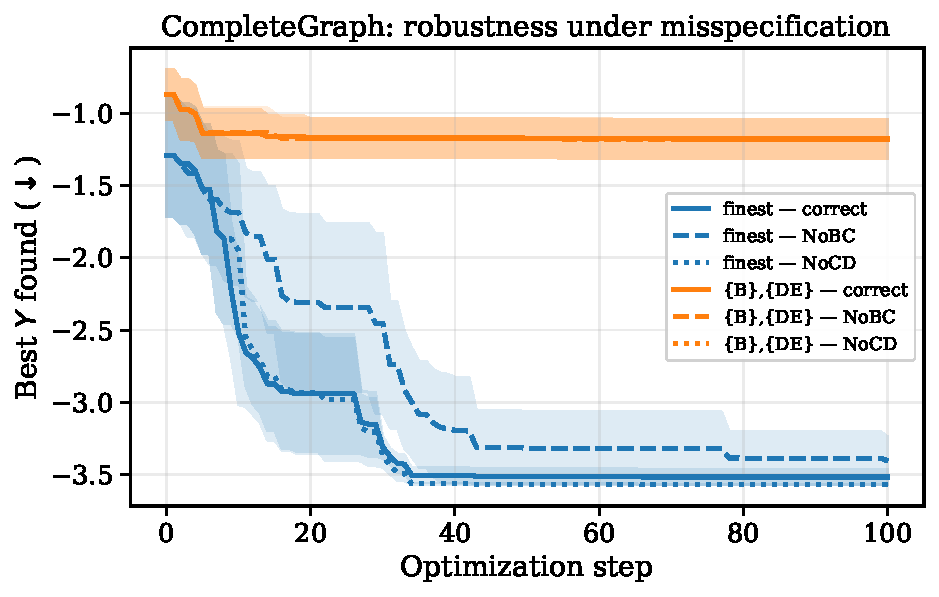
\includegraphics[width=0.49\textwidth]{figures/CompleteGraph_wrong_edge.pdf}
  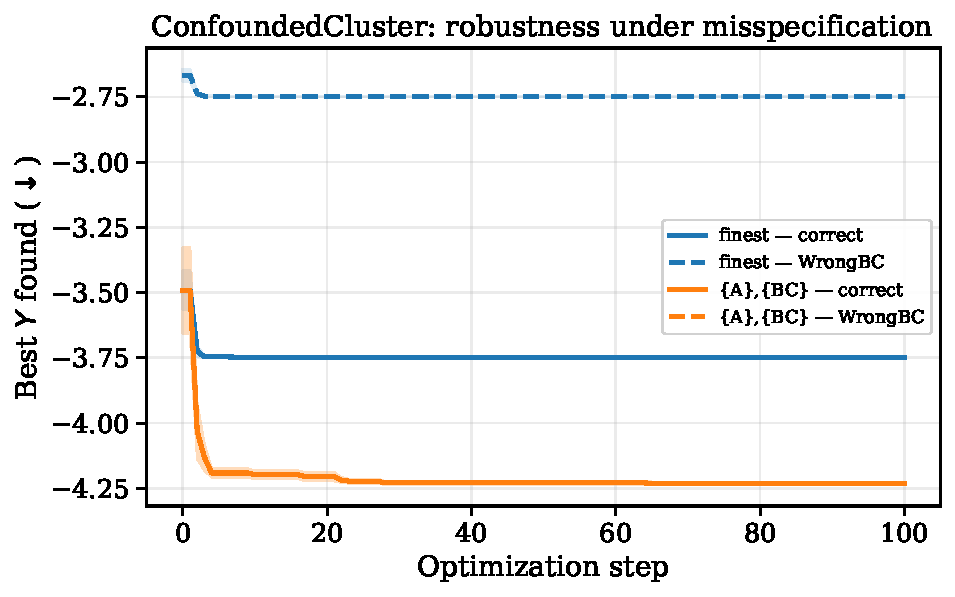
\includegraphics[width=0.49\textwidth]{figures/ConfoundedCluster_wrong_edge.pdf}
  \caption{Robustness under misspecification (best-so-far $Y$, mean $\pm$ s.e.):
  Tier-1 prior bias on CompleteGraph (left) and Tier-2 arm deletion on the
  ConfoundedCluster bow benchmark (right). Colour = partition, solid = correct
  DAG, dashed = misspecified DAG. At the coarse partition the misspecified and
  correct curves coincide (Prop.~\ref{prop:invariance}); at the finest
  partition the bow benchmark's \texttt{WrongBC} curve is strictly worse,
  reflecting the deleted optimal target.}
  \label{fig:robustness}
\end{figure}


% ==========================================
\section{Discussion}
\label{sec:discussion}

\begin{itemize}[leftmargin=1.2em,itemsep=1pt,topsep=2pt]
  \item Prop.~\ref{prop:invariance} is structural, not statistical:
  coarsening acts as a hard regularizer on the hypothesis space, trading
  resolution (Prop.~\ref{prop:price}) for immunity to an entire class of
  misspecifications. The practitioner chooses where on this dial to sit by
  choosing how much structure to commit to.
  \item The damage taxonomy (Remark~\ref{rem:taxonomy}) reframes "is CBO
  robust to a wrong graph?": prior bias is self-healing under any
  reasonable acquisition; arm damage is not. Robustness analyses that only
  perturb priors miss the failure mode that matters.
  \item The partition need not be guessed once and forever:
  Prop.~\ref{prop:refinement} makes refinement monotonically safe
  (identifiable arms are never lost), although validity must be re-checked
  (Prop.~\ref{prop:refinement_validity}). Discovering the partition online
  from interventional data --- e.g.\ with the RePaRe routine of
  \citet{madaleno2026coarsening} --- is a natural recursive extension that
  we develop in follow-up work.
\end{itemize}

\section{Limitations}
\label{sec:limitations}

(i) The gated design (Eq.~\ref{eq:es_gate}) commits to the assumed
structure; the un-gated variant (explore non-identified arms under an
uninformative prior) converts arm damage into exploration overhead and
deserves a systematic comparison. (ii) The GP estimator cascade behind
Eq.~\eqref{eq:two_tier_prior} is sound but not complete
(Assumption~\ref{ass:id_scheme}). (iii) We evaluate on the curated
hard-intervention subset of the \textsc{CausalBO} benchmark plus a
purpose-built confounded-cluster benchmark; soft-intervention /
function-network settings are out of scope (\QCBO{} is a hard-intervention
method). (iv) Our latent projection handles the bidirected structure these
benchmarks exhibit; bidirected-input projection through drop-only chains is
not implemented (it does not arise here), so the ``absorbs latent
confounding'' claim is scoped to that setting. (v) Faithfulness does not
transfer to the cluster level \citep{wahl2024foundations}, so cluster-level
conditional independences observed in data must not be read back as
fine-grained structure. (vi) We evaluate at unit intervention costs;
cost-asymmetric settings change where coarsening pays. (vii) The benchmark's
oracle optima $y^*$ are extreme reference values --- in some datasets attained
by interventions outside the domain the methods search (e.g.\ Epidemiology,
whose reported optimizer lies far outside the interventional ranges) --- so the
absolute GAP is uniformly deflated across all methods; we therefore read GAP and
PA-GAP as relative rankings, not attainment fractions, and locate \QCBO{}'s
contribution in the robustness and price analyses rather than in benchmark GAP
magnitudes.

\section{Conclusion}
\label{sec:conclusion}

\QCBO{} makes causal Bayesian optimization usable at the level of
structural knowledge practitioners actually have --- clusters --- with a
complete identification gate, a provable invariance to intra-cluster
misspecification, and an exact characterization of what coarseness costs.
On the spectrum from structure-free \BO{} to oracle-graph \CBO{}, it
provides the missing, principled middle; refining the partition as
evidence accumulates closes the remaining gap and is the subject of
ongoing work.


% ==========================================
\appendix

\section{Benchmark datasets and partitions}
\label{app:datasets}

For each curated \textsc{CausalBO} dataset we run \QCBO{} at the identity
partition (\QCBO{}-finest $\equiv$ \CBO{}, Prop.~\ref{prop:identity}) and at one
domain-meaningful coarse partition. The coarse partition groups manipulable
variables a practitioner would lump into a subsystem without committing to the
edges \emph{within} it; validity (acyclicity of the quotient) is checked
automatically (Assumption~\ref{ass:valid}). Table~\ref{tab:partitions} lists
the manipulable set and the coarse partition per dataset; the DAGs are read
from each dataset's structural equations.
Figures~\ref{fig:dag-toygraph}--\ref{fig:dag-confounded} draw each dataset's
fine-grained ADMG beside its quotient C-DAG. Throughout, solid arrows denote
directed causes and dashed red double arrows denote latent confounders
(bidirected edges); the target $Y$ is gold, manipulable variables orange, other
observables blue, and a rounded box marks a quotient cluster of more than one
variable.

\begin{table}[h]
  \centering
  \caption{Curated benchmark datasets: manipulable variables and the coarse
  partition used (the identity partition is always also run). $Y$ is the
  target; non-manipulable observables remain atomic singletons of the
  quotient.}
  \label{tab:partitions}
  \vspace{4pt}
  \small
  \begin{tabular}{@{}llll@{}}
    \toprule
    \textbf{Dataset} & \textbf{Manipulable} & \textbf{Coarse partition} &
    \textbf{Rationale} \\
    \midrule
    ToyGraph / Synthetic-2 & $\{X,Z\}$ & $\{X,Z\}$ & absorb the chain $X\to Z$ \\
    Synthetic (CompleteGraph) & $\{B,D,E\}$ & $\{B\},\{D,E\}$ & $D,E$ are the output stage \\
    Healthcare & \{Aspirin, Statin\} & \{Aspirin, Statin\} & one ``medication'' lever \\
    Epidemiology & $\{L,B\}$ & $\{L,B\}$ & joint exposure \\
    Ecology & $\{N,O,C,T,D\}$ & $\{C,N,O\},\{D,T\}$ & nutrient/chemistry vs.\ temperature/depth \\
    \midrule
    ConfoundedCluster (bow) & $\{A,B,C\}$ & $\{A\},\{B,C\}$ & confounded pair $B,C$ \\
    \bottomrule
  \end{tabular}
\end{table}

\newcommand{\dagpair}[1]{%
  \begin{subfigure}{0.46\textwidth}\centering
    \includegraphics[width=\linewidth,height=5.4cm,keepaspectratio]{figures/#1_dag.pdf}
    \caption{Fine-grained ADMG}
  \end{subfigure}\hfill
  \begin{subfigure}{0.46\textwidth}\centering
    \includegraphics[width=\linewidth,height=5.4cm,keepaspectratio]{figures/#1_cdag.pdf}
    \caption{Quotient C-DAG}
  \end{subfigure}}

\begin{figure}[ht]
  \centering
  \dagpair{ToyGraph}
  \caption{\textbf{ToyGraph / Synthetic-2.} The chain $X\to Z\to Y$. Merging the
  manipulable variables into one cluster $\{X,Z\}$ leaves a single quotient edge
  $\{X,Z\}\to Y$.}
  \label{fig:dag-toygraph}
\end{figure}

\begin{figure}[ht]
  \centering
  \dagpair{Synthetic}
  \caption{\textbf{Synthetic (CompleteGraph).} Latent confounders $U_1\to\{A,Y\}$
  and $U_2\to\{B,Y\}$ appear as the bidirected edges $A\leftrightarrow Y$ and
  $B\leftrightarrow Y$. Coarsening the output stage $\{D,E\}$ does not touch
  these confounders---they cross cluster boundaries---so both survive in the
  C-DAG.}
  \label{fig:dag-synthetic}
\end{figure}

\begin{figure}[ht]
  \centering
  \dagpair{Healthcare}
  \caption{\textbf{Healthcare.} Age and BMI confound the two medication levers,
  the cancer mediator, and the outcome (no latent confounders). The coarse
  partition merges Aspirin and Statin into a single ``medication'' cluster.}
  \label{fig:dag-healthcare}
\end{figure}

\begin{figure}[ht]
  \centering
  \dagpair{Epidemiology}
  \caption{\textbf{Epidemiology.} Treatment $T$ drives the exposures $\{L,B\}$,
  the mediator $R$, and the outcome. The coarse partition treats the joint
  exposure $\{L,B\}$ as one lever.}
  \label{fig:dag-epidemiology}
\end{figure}

\begin{figure}[ht]
  \centering
  \dagpair{Ecology}
  \caption{\textbf{Ecology.} The largest curated graph. The quotient cluster
  $\{D,T\}$ has \emph{no} directed path to $Y$ ($D$ is a pure sink and $T$ is
  isolated): the practitioner-chosen grouping cleanly isolates a subsystem
  irrelevant to the objective.}
  \label{fig:dag-ecology}
\end{figure}

\begin{figure}[ht]
  \centering
  \dagpair{ConfoundedCluster}
  \caption{\textbf{ConfoundedCluster (bow).} The latent confounder over the pair
  $\{B,C\}$ is a \emph{bow}: the bidirected edge $B\leftrightarrow C$. Once
  $\{B,C\}$ is a single cluster the bow becomes intra-cluster and is projected
  out---the C-DAG carries \emph{no} bidirected edge, the structural mechanism
  behind the within-cluster invariance of Prop.~\ref{prop:invariance}.}
  \label{fig:dag-confounded}
\end{figure}


% ==========================================
\section{Proofs}
\label{app:proofs}

The main text (\S\ref{sec:theory}) states each result with a short sketch;
here are the full proofs. Notation is as in \S\ref{sec:setup} and
\S\ref{sec:theory}.

\begin{proof}[Proof of Prop.~\ref{prop:identity}]
Singleton clusters make the quotient map the identity on $\Gg^{*}$, and
unions of at most $m$ singletons are exactly the subsets of size at most
$m$.
\end{proof}

\begin{proof}[Proof of Prop.~\ref{prop:invariance}]
The latent projection removes only latent vertices; an edge between two
observables is never an interior vertex of a projection path, so
$(\Gg')^{*}$ and $\Gg^{*}$ differ exactly by the modified intra-cluster
edges. The quotient keeps a directed (resp.\ bidirected) cluster-level
edge iff some fine edge crosses two \emph{distinct} clusters; edges within
a cluster contribute nothing. Hence the quotients coincide. All remaining
objects --- $\ESpi$, ID formulas, priors --- are functions of $\Gq$ and
data alone.
\end{proof}

\begin{proof}[Proof of Prop.~\ref{prop:refinement_validity}]
Take $\mathbf{X}=\{a_1,a_2,b_1,b_2\}$ with fine edges $a_1\to b_1$ and
$b_2\to a_2$. The coarsest partition $\pi=\{\{a_1,a_2,b_1,b_2\}\}$ is valid:
both edges are intra-cluster, so the quotient has a single manipulable node
and is acyclic. Its refinement $\pi'=\{\{a_1,a_2\},\{b_1,b_2\}\}$ exposes both
edges as inter-cluster --- $a_1\to b_1$ contributes $A\to B$ and $b_2\to a_2$
contributes $B\to A$ --- inducing the 2-cycle $A\rightleftarrows B$, so
$\mathcal{G}^{\pi'}$ is cyclic and $\pi'$ is invalid. Decidability is immediate
from the acyclicity clause of Def.~\ref{def:coarsening}.
\end{proof}

\begin{proof}[Proof of Prop.~\ref{prop:refinement}]
(i) A union of $\pi$-clusters is a union of $\pi'$-clusters because each
$\pi$-cluster is. (ii) Quotienting is compositional: $\Gq$ is the quotient
of $\mathcal{G}^{\pi'}$ under the induced partition of $\pi'$-clusters, so
every fine graph compatible with $\mathcal{G}^{\pi'}$ is compatible with
$\Gq$. Identifiability from $\Gq$ means a single functional of the
observational distribution equals $\E[Y \mid \do(S)]$ across all SCMs
whose graph is compatible with $\Gq$ \citep{anand2023cdag}; a fortiori the
same functional works across the smaller class compatible with
$\mathcal{G}^{\pi'}$.
\end{proof}

\begin{proof}[Proof of Prop.~\ref{prop:price}]
By Prop.~\ref{prop:refinement}(i), $\ESpi_0 \subseteq
\mathfrak{S}^{\pi'}_0 \subseteq \mathfrak{S}^{\pi_\top}_0 =
2^{\mathbf{X}}\setminus\{\emptyset\}$; minima over larger sets are no
larger. Equality holds iff the unrestricted argmin intersects $\ESpi_0$,
which is exactly the stated condition.
\end{proof}


% ==========================================
\bibliographystyle{abbrvnat}
\begin{thebibliography}{24}

\bibitem[Anand et al.(2023)]{anand2023cdag}
T.~V.~Anand, A.~H.~Ribeiro, J.~Tian, and E.~Bareinboim.
\newblock Causal effect identification in cluster {DAG}s.
\newblock In \emph{AAAI}, volume 37, pp.\ 12172--12179, 2023.

\bibitem[Aglietti et al.(2020)]{aglietti2020causal}
V.~Aglietti, X.~Lu, A.~Paleyes, and J.~Gonz{\'a}lez.
\newblock Causal {B}ayesian optimization.
\newblock In \emph{AISTATS}, volume 108 of \emph{PMLR}, pp.\ 3155--3164, 2020.

\bibitem[Aglietti et al.(2021)]{aglietti2021dynamic}
V.~Aglietti, N.~Dhir, J.~Gonz{\'a}lez, and T.~Damoulas.
\newblock Dynamic causal {B}ayesian optimization.
\newblock In \emph{NeurIPS}, volume 34, 2021.

\bibitem[Aglietti et al.(2023)]{aglietti2023constrained}
V.~Aglietti, A.~Malek, I.~Ktena, and S.~Chiappa.
\newblock Constrained causal {B}ayesian optimization.
\newblock In \emph{ICML}, 2023.

\bibitem[Beckers \& Halpern(2019)]{beckers2019approximate}
S.~Beckers and J.~Y.~Halpern.
\newblock Abstracting causal models.
\newblock In \emph{AAAI}, 2019.

\bibitem[Branchini et al.(2023)]{branchini2023causal}
N.~Branchini, V.~Aglietti, N.~Dhir, and T.~Damoulas.
\newblock Causal {B}ayesian optimization via local causal discovery.
\newblock In \emph{CLeaR}, volume 236 of \emph{PMLR}, 2023.

\bibitem[Ferreira \& Assaad(2025)]{ferreira2025cdmg}
E.~Ferreira and C.~K.~Assaad.
\newblock Identifying macro causal effects in a {C-DMG} over {ADMG}s.
\newblock \emph{arXiv:2504.01551}, 2025.

\bibitem[Gamella et al.(2025)]{gamella2025chamber}
J.~L.~Gamella, J.~Peters, and P.~B{\"u}hlmann.
\newblock Causal chambers as a real-world physical testbed for {AI}
methodology.
\newblock \emph{Nature Machine Intelligence}, 7:107--118, 2025.

\bibitem[Garnett(2023)]{garnett2023bayesian}
R.~Garnett.
\newblock \emph{Bayesian Optimization}.
\newblock Cambridge University Press, 2023.

\bibitem[Lee et al.(2023)]{lee2023ananke}
J.~J.~R.~Lee, R.~Bhattacharya, R.~Nabi, and I.~Shpitser.
\newblock Ananke: A python package for causal inference using graphical
models.
\newblock \emph{arXiv:2301.11477}, 2023.

\bibitem[Lee \& Bareinboim(2018)]{lee2018structural}
S.~Lee and E.~Bareinboim.
\newblock Structural causal bandits: Where to intervene?
\newblock In \emph{NeurIPS}, 2018.

\bibitem[Lee et al.(2019)]{lee2019latent}
S.~Lee, J.~Correa, and E.~Bareinboim.
\newblock General identifiability with arbitrary surrogate experiments.
\newblock In \emph{UAI}, 2019.

\bibitem[Madaleno et al.(2026)]{madaleno2026coarsening}
F.~Madaleno, P.~Misra, and A.~Markham.
\newblock Coarsening causal {DAG} models.
\newblock \emph{arXiv:2601.10531}, 2026.

\bibitem[Mukherjee et al.(2024)]{mukherjee2024gacbo}
S.~Mukherjee, et al.
\newblock Graph-agnostic causal {B}ayesian optimization.
\newblock \emph{arXiv}, 2024.

\bibitem[Park et al.(2025)]{park2025dmis}
J.~Park, M.~Zemplenyi, and V.~Aglietti.
\newblock Causal {B}ayesian optimization under partial observability.
\newblock \emph{arXiv}, 2025.

\bibitem[Pearl(2009)]{pearl2009causality}
J.~Pearl.
\newblock \emph{Causality: Models, Reasoning and Inference}.
\newblock Cambridge University Press, 2nd edition, 2009.

\bibitem[Poloczek et al.(2017)]{poloczek2017multi}
M.~Poloczek, J.~Wang, and P.~Frazier.
\newblock Multi-information source optimization.
\newblock In \emph{NeurIPS}, 2017.

\bibitem[Shpitser \& Pearl(2006)]{shpitser2006identification}
I.~Shpitser and J.~Pearl.
\newblock Identification of joint interventional distributions in
recursive semi-{M}arkovian causal models.
\newblock In \emph{AAAI}, 2006.

\bibitem[Sussex et al.(2023)]{sussex2023model}
S.~Sussex, A.~Makarova, and A.~Krause.
\newblock Model-based causal {B}ayesian optimization.
\newblock In \emph{ICLR}, 2023.

\bibitem[Tikka et al.(2025)]{tikka2025relaxing}
Anonymous.
\newblock Relaxing partition admissibility in cluster-{DAG}s: a causal
calculus with arbitrary variable clustering.
\newblock \emph{arXiv:2511.01396}, 2025.
% TODO: fix author list from the arXiv page before submission.

\bibitem[Wahl et al.(2024)]{wahl2024foundations}
J.~Wahl, U.~Ninad, and J.~Runge.
\newblock Foundations of causal discovery on groups of variables.
\newblock \emph{Journal of Causal Inference}, 12(1), 2024.

\bibitem[Wang et al.(2025)]{ll2025cdagdiscovery}
Anonymous.
\newblock Cluster-{DAG}s as powerful background knowledge for causal
discovery.
\newblock \emph{arXiv:2512.10032}, 2025.
% TODO: fix author list from the arXiv page before submission.

\bibitem[Zeitler(2025)]{zeitler2025mfacbo}
J.~Zeitler.
\newblock Towards {MFACBO}: Multi-fidelity abstraction causal {B}ayesian
optimization.
\newblock In \emph{1st Workshop on Causal Abstractions and Representations
(CAR) at UAI}, 2025.

\bibitem[Tian \& Pearl(2002)]{tian2002general}
J.~Tian and J.~Pearl.
\newblock A general identification condition for causal effects.
\newblock In \emph{AAAI}, 2002.

% ---- STUBS (replace in the bibliography pass) ----
\bibitem[Anonymous(2026)]{anonymous2026cbobench}
Anonymous.
\newblock Causal {B}ayesian optimization: Foundations, methods, and applications.
\newblock Under review, 2026. % TODO: fill from OpenReview XT6DC37m5I.

\bibitem[Durand et al.(2025)]{durand2025unknown}
J.~Durand, Y.~Annadani, S.~Bauer, and S.~Parbhoo.
\newblock Causal {B}ayesian optimization with unknown causal graphs.
\newblock In \emph{ICLR}, 2025. % TODO: verify author list / venue details.

\bibitem[Arsenyan et al.(2026)]{arsenyan2026contextual}
V.~Arsenyan, A.~Grosnit, H.~Bou~Ammar, and A.~S.~Dalalyan.
\newblock Contextual causal {B}ayesian optimisation.
\newblock In \emph{ICLR}, 2026. % TODO: verify details.

\end{thebibliography}

\end{document}
